\documentclass{article}

\usepackage{KjelsethReportStyle}

%   ############################## Customisation ##############################

% Document metadata
\title{\fontsize{24}{36}\selectfont PB1180 - Programmerbare logiske kretser\\ %Edit title here \\ means new line
Final Project} % Line 2 of title, its not subtitle, that is possible to, google it
\author{{\Large\normalfont Kandidatnr:}\\
{\Large\ttfamily 8022}} % Input your name, replace \ttfamily with \normalfont to make it not monospaced but regular font (removing \ttfamily will not do this because of the monospaced font inside tables command, and author is technically a 1x1 table)
\date{\today} % Auto updates the date, untill you export it, replace with hardcoded date if you need

%   ############################## Document begins here ##############################
\begin{document}

\maketitle % Makes title front page based on the title, author and date metadata, change at the top
% Logo
\begin{tikzpicture}[remember picture,overlay]
   \node[anchor=north west,inner sep=35pt] at (current page.north west)
              {
\includegraphics[scale=0.3]{Figures/usnlogo.png}};
\end{tikzpicture}


%   ############################## Section ##############################
\addtocontents{toc}{\protect\setcounter{tocdepth}{0}} % Temporarily hide from TOC
\section{Abstract} % Numbered section named Introduction
This is the report for the Final Project in PB-1180 - Programmerbare logiske kretser. There were two possible mutually exclusive projects to choose from and I chose to do Course Project B. There were given no criteria for report formatting, therefore it does not follow any given template and is customized to my own liking. \par
Programs used to complete this project:
\begin{itemize}
    \item Visual Studio Code - as a general code writing editor 
    \item VHDL by VHDLwhiz plug-in for VScode - for syntax highlighting
    \item GitHub - private repository to store code and figures for synchronizing
    \item ModelSim - to simulate using test benches 
    \item Quartus - for implementation on FPGA and synthesizing RTL views 
    \item Excel - to write tables used in the report
    \item Excel2LaTeX Excel add-inn - to generate \LaTeX code from Excel table
    \item SmartDraw - for making state transition diagram
    \item Affinity Photo 2 - to edit/crop photos for the report
    \item DaVinci Resolve 20 - for editing the included video
    \item Overleaf - to write the report using \LaTeX
\end{itemize}


\clearpage
\tableofcontents % Generate TOC
%\hfill
\clearpage
\listoffigures % List of figures
\hfill
\listoftables % List of tables
\addtocontents{toc}{\protect\setcounter{tocdepth}{2}} % Restore TOC depth



%   ############################## Section ##############################
\section{Approach to solution}
\subsection{Introduction}
My approach for a Project like this is to start by systematically segment it to smaller tasks. I started by writing a top level overview of how I want this report to be structured and then I started dissecting the problem. After the problem was understood I started with figuring out how I would like to solve the problem. Then after a high level overview of the solution is made I created a structure where I can write the code to be readable and easily understandable. Then it was onto actually writing the code, here Lab exercise 5 and 6 taught me a lot about the principals used in this project and a lot of the code is inspired from my completion of those. After the code was completed I first tested it on the FPGA, where it worked, and then later developed test benches to simulate. This is mostly because I was very certain that the logic was good and only thing that could be wrong would be some minor issues that could easily be fixed. In the end I started making this report, editing the photos and videos, and including them. And finally the report is written.
\subsection{The Problem}
To solve the problem presented in the task, the problem must first be understood at the basic level. When the problem is acknowledged a solution can be formed. The stated problem, in simplified form, is to make a circuit that can serially display a certain combination of blinks encoded to be interpreted as some characters. With some additional details, such as a reset button with light and a 7 segment display of the character.
\subsection{Definitions}
To avoid confusion these definitions and acronyms will be used:
\begin{itemize}
    \item Letters - is  all the characters the code will display, P, B, 1, 8, -, and so on
    \item Symbols - is the type of signal that makes up a character, dot, dash and bar
    \item FSM - Finite State Machine
    \item TLE - Top level entity
    \item FPGA - Field-Programmable Gate Array
    \item HDL - Hardware Descriptive Language
    \item VHDL - Very High Speed Integrated Circuit HDL
\end{itemize}
\clearpage
\subsection{Solving}\label{section:solving}
The first thing to realize when solving is that this is very similar to morse code. The exception is that morse code is only two symbols, dot and dash, and the gamma code has the extra vertical bar symbol. In addition one dot is 4 short pulses instead of a singular short pulse like in morse code. To solve this task it is good to start with the encoding. At any point during transmission the LED can only be in two states, on or off. This means it is possible to encode each character as a string of ones and zeros with each bit representing the state for a short time. This will make a code with little logic and a large lookup table. I felt this would have been a bad design and chose not to do it this way. Instead the encoding was made for each possible symbol that describes a letter. These three values they can be represented with two bits. 01 for dot, 10 for dash and 11 for bar. This leaves 00 free and used this encoding for the pause between each symbol. Using this encoding set, a FSM was designed as described in \ref{section:FSM}. A lot of the code I made was inspired by the code I made for Lab 05. Some parts of the code was copy pasted but most parts were redesigned for better readability and to fit the bigger letter encoding.
\subsection{Structure}
For better readability it was coded into 4 separate components:
\begin{enumerate}
    \item Lookup table - for letter selection
    \item Shift Register - for storing current Letter and shifting it along
    \item Decoder - for the 7 segment display
    \item Logic control - for the FSM transitions and output
\end{enumerate}
Then the TLE connects all together and does not contain any logic except for a startup reset and the Reset button LED.

%   ############################## Section ##############################
\section{The FSM}
\subsection{State logic design}\label{section:FSM}
 Using the encoding described in \ref{section:solving} a FSM diagram was started, where Dot, Dash, Bar and Between are 4 states. in addition the system needed a default state it can reset to and not show anything, this is the Idle state. The Dot, Dash, Bar and Between state could branch out from Idle directly, but that makes the transition logic cumbersome as then all states need to be able to go directly to all other states. Instead a segway state for controlling the timers and routing the states was made, the Running state. This state will only be on for a single clock cycle but does all of the routing logic. After this initial plan a modification to the Dot state was made. It is split into two states, a Dot On and Dot Off, where it alternates between to blink on 4 times before returning to Running. With the states set up like this the output was very simple, only depending on what state it was in, nothing else. In table~\ref{tab:StateTransition} The state transitions is described in detail. Based on the current state (Columns) the next state will be the listed one based on if the input value (Rows) is true, a "-" signifies no state change. Obviously this table can't contain all possible values and still be readable so all non listed values will result in no state change. If this table seems the wrong way around it is because it is transposed to be able to fit the document. Table~\ref{tab:StateOutput} describes the outputs, and because the choice of states it is very simple and only relies on the current state. Note that Display or Load is redundant as they are just opposite, both are included for readability, not out of necessity. There are multiple ways to encode the state variable and the Task specifies to use "my preferred encoding method" and as I am not making any structural logic for the states it does not affect anything whatever the encoding is. When compiling the code in Quartus the encoding used is one-hot as shown in figure~\ref{fig:StateEncoding}.
\hspace{3cm}
\begin{figure}[h]
    \centering
    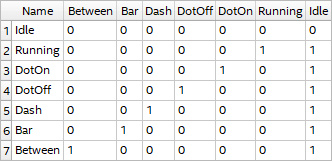
\includegraphics[width=0.7\textwidth]{Figures/State encoding.jpg}
    \figcaption{Encoding table made by Quartus}
    \label{fig:StateEncoding}
\end{figure}

\clearpage

\begin{figure}[h]
    \centering
    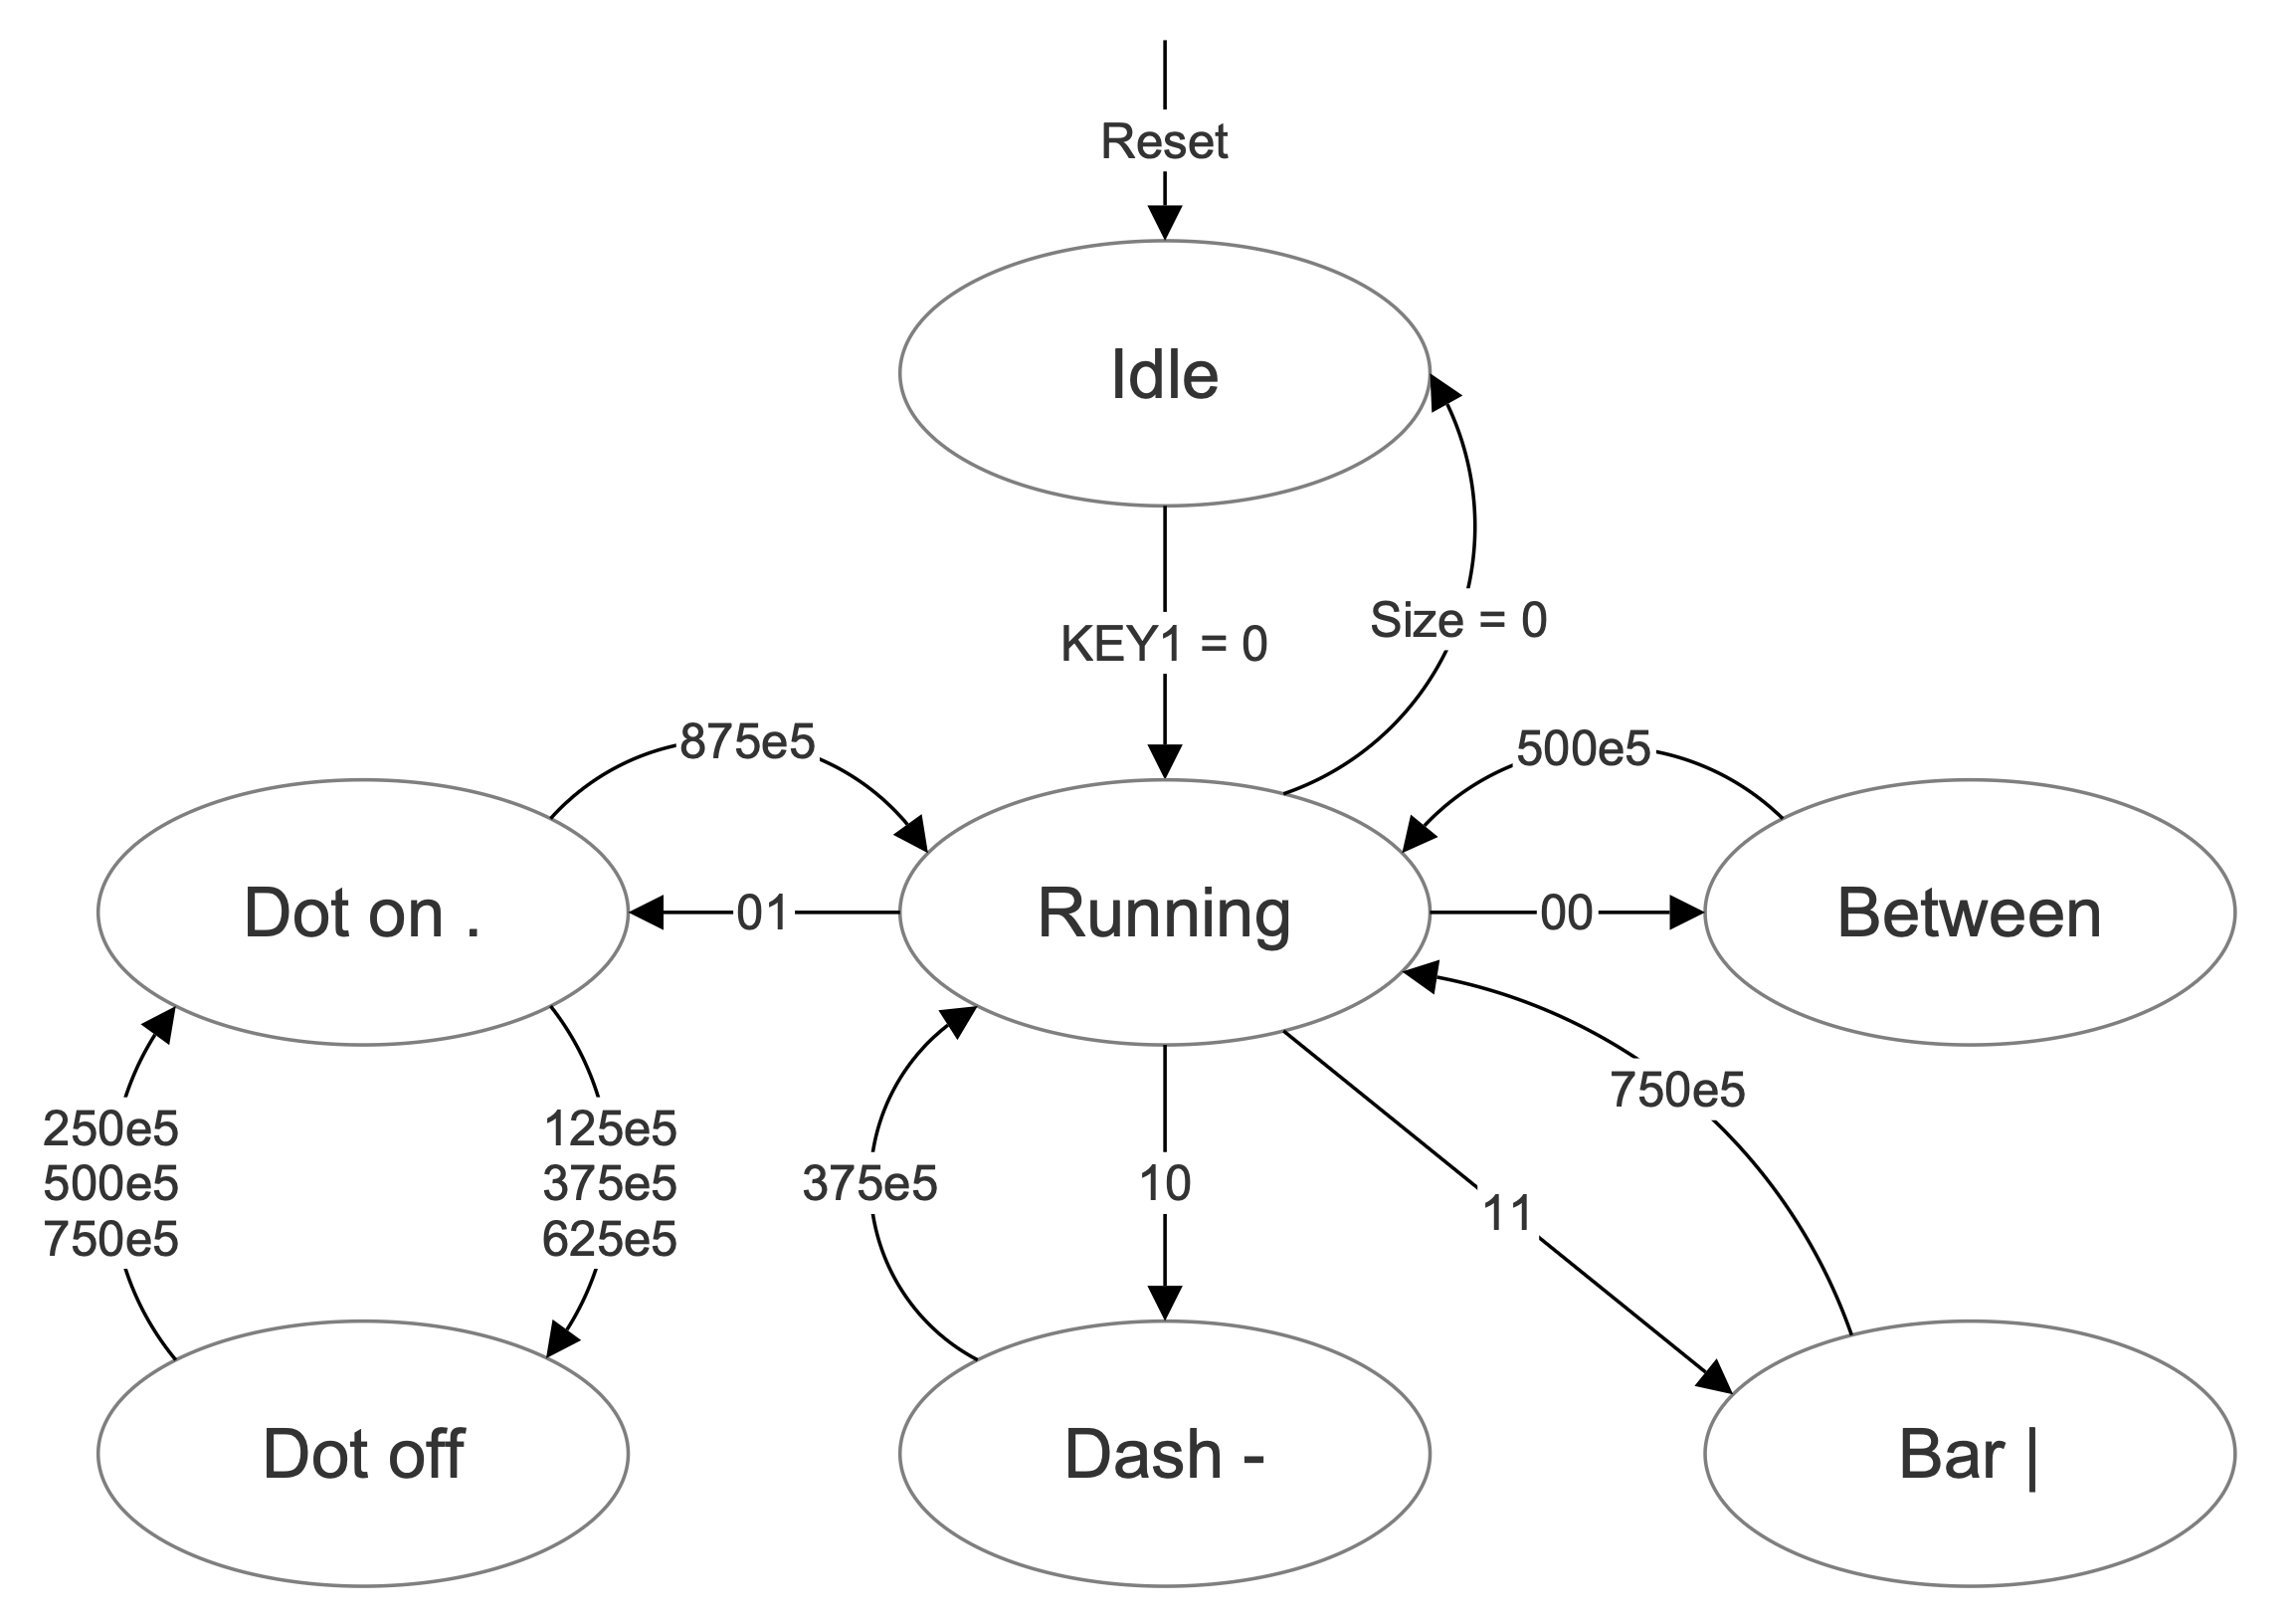
\includegraphics[width=1\textwidth]{Figures/StateTransitionDiagram.png}
    \figcaption{State transition diagram}
    \label{fig:StateTransition}
\end{figure}
In this diagram the numbers with the e5 suffix is representing the counter value and the two digit numbers is representing the value of the two most significant bits of the letter data. Dot on and Dot off have 3 different values where the state jump between them.

\clearpage
 \subsection{State tables}
 
% Table generated by Excel2LaTeX from sheet 'States'
\begin{table}[htbp]
  \centering
  \caption{State transitions}
    \resizebox{\textwidth}{!}{%
    \begin{tabular}{|c|c|c|c|c|c|c|c|c|c|}
    \hline
    \multicolumn{3}{|c|}{\multirow{2}[4]{*}{\textbf{State transition}}} & \multicolumn{7}{c|}{\textbf{Current state}} \bigstrut\\
\cline{4-10}    \multicolumn{3}{|c|}{} & \multicolumn{1}{l|}{\textbf{Idle}} & \multicolumn{1}{l|}{\textbf{Running}} & \multicolumn{1}{l|}{\textbf{DotOn}} & \multicolumn{1}{l|}{\textbf{DotOff}} & \multicolumn{1}{l|}{\textbf{Dash}} & \multicolumn{1}{l|}{\textbf{Bar}} & \multicolumn{1}{l|}{\textbf{Between}} \bigstrut\\
    \hline
    \textbf{Input} & \textbf{Type} & \textbf{Value} & \textbf{S0} & \textbf{S1} & \textbf{S2} & \textbf{S3}    & \textbf{S4}    & \textbf{S5}    & \textbf{S6} \bigstrut\\
    \hline
    \multirow{2}[4]{*}{\textbf{Keys}} & \textbf{Reset} & \textbf{KEY0 = 0} & S0    & S0    & S0    & S0    & S0    & S0    & S0 \bigstrut\\
\cline{2-10}          & \textbf{Load} & \textbf{KEY1 = 0} & S1    & -     & -     & -     & -     & -     & - \bigstrut\\
    \hline
    \multirow{5}[10]{*}{\textbf{Letter}} & \textbf{Size} & \textbf{Size = 0} & -     & S0    & -     & -     & -     & -     & - \bigstrut\\
\cline{2-10}          & \textbf{Between} & \textbf{00} & -     & S6    & -     & -     & -     & -     & - \bigstrut\\
\cline{2-10}          & \textbf{Dot} & \textbf{01} & -     & S2    & -     & -     & -     & -     & - \bigstrut\\
\cline{2-10}          & \textbf{Dash} & \textbf{10} & -     & S4    & -     & -     & -     & -     & - \bigstrut\\
\cline{2-10}          & \textbf{Bar} & \textbf{11} & -     & S5    & -     & -     & -     & -     & - \bigstrut\\
    \hline
    \multirow{7}[14]{*}{\textbf{Counter}} & \textbf{0.25s} & \textbf{125e5} & -     & -     & S3    & -     & -     & -     & - \bigstrut\\
\cline{2-10}          & \textbf{0.5s} & \textbf{25e6} & -     & -     & -     & S2    & -     & -     & - \bigstrut\\
\cline{2-10}          & \textbf{0.75s} & \textbf{375e5} & -     & -     & S3    & -     & S1    & -     & - \bigstrut\\
\cline{2-10}          & \textbf{1s} & \textbf{5e7} & -     & -     & -     & S2    & -     & -     & S1 \bigstrut\\
\cline{2-10}          & \textbf{1.25s} & \textbf{625e5} & -     & -     & S3    & -     & -     & -     & - \bigstrut\\
\cline{2-10}          & \textbf{1.5s} & \textbf{75e6} & -     & -     & -     & S2    & -     & S1    & - \bigstrut\\
\cline{2-10}          & \textbf{1.75s} & \textbf{875e5} & -     & -     & S1    & -     & -     & -     & - \bigstrut\\
    \hline
    \end{tabular}}%
  \label{tab:StateTransition}%
\end{table}%

% Table generated by Excel2LaTeX from sheet 'States'
\begin{table}[htbp]
  \centering
  \caption{State outputs}
    \begin{tabular}{|l|c|c|c|c|c|}
    \hline
    \multicolumn{2}{|c|}{\textbf{State output}} & \multicolumn{4}{c|}{\textbf{Outputs}} \bigstrut\\
    \hline
    \multicolumn{2}{|c|}{\textbf{Current state}} & \textbf{LED} & \textbf{Display} & \textbf{Shift} & \textbf{Load} \bigstrut\\
    \hline
    \textbf{Idle} & \textbf{S0} & 0     & 0     & 0     & 1 \bigstrut\\
    \hline
    \textbf{Running} & \textbf{S1} & 0     & 1     & 0     & 0 \bigstrut\\
    \hline
    \textbf{Dot} & \textbf{S2} & 1     & 1     & 1     & 0 \bigstrut\\
    \hline
    \textbf{Dot off} & \textbf{S3}    & 0     & 1     & 1     & 0 \bigstrut\\
    \hline
    \textbf{Dash} & \textbf{S4}    & 1     & 1     & 1     & 0 \bigstrut\\
    \hline
    \textbf{Bar} & \textbf{S5}    & 1     & 1     & 1     & 0 \bigstrut\\
    \hline
    \textbf{Between} & \textbf{S6}    & 0     & 1     & 1     & 0 \bigstrut\\
    \hline
    \end{tabular}%
  \label{tab:StateOutput}%
\end{table}%

\subsection{Moore and Mealy}
Comparing this design with the fundamental Moore and Mealy machines it is very clear that this is a Moore machine. The main reasoning is that the outputs only depend on the current state. The reason for doing this is very simple, Moore machines are easier to make than Mealy machines. As this design is not very large anyway, in the context of this task, it seems unreasonable to focus on the optimization possible with a Mealy machine. The number of states and logic is not large enough to see any real improvements. It is worth noting that the 1 clock cycle output delay a Moore machine has can be seen in the simulation result in figure~\ref{fig:TB_Logic}. This delay is because on the first clock cycle the State changes, then on the next clock cycle the output changes.

%   ############################## Section ##############################
\section{VHDL code}

\subsection{FSM code}
\writecode[VHDL]{FinalProject.vhd}{TLE that ties the system together}
Originally LED0 was the chosen output LED, but after trying to film and realizing LED0 is under the label I chose LED3 as it is directly under the used 7 segment display. For the Light on reset I simply not gated the reset button and used LED2 next to the output LED. LEDs 9 to 4 and 1 to 0 is not used and therefore constant low, if this was not set the LED would appear half on in an undefined state and that looks bad and could be confusing.
\writecode[VHDL]{LetterSelection.vhd}{Letter selector is a lookup table}
The Letter data is simply a string of the symbols that make up each letter. Then between each symbol 00 is inserted to have the wait in-between each symbol being displayed. Technically this could have been omitted and only the symbol part being part of the string, but this would make the state transitions unnecessary more complex. the string is always 14 bits, which would be a size of maximum 7 symbols and betweens. For the letters not using 4 symbols the remaing string is filled with "-" which is the don't care signal.
\clearpage
\writecode[VHDL]{LetterRegister.vhd}{Custom loadable shift register}
The shift register shifts two bits each time shift is enabled, causing the two most significant bits to be the next symbol or between for the logic to read. It shifts in two don't care signals as it doesn't matter what it resolves to, it is never read. it also subtracts the size of the letter by one at the same time. Both Load and LetterLoad is needed in the sensitivity list. This is because if the switches don't change after going into idle, Load needs to trigger the register to update the to current selected letter, and if the current selection changes while in idle LetterLoad will change and therefore update the process and update the output letter.
\clearpage
\writecode[VHDL]{Decoder7Segment.vhd}{Decoder with load for 7-segment display output}
The decoder is simply a lookup table that outputs the loaded symbol to the display whenever enabled. The stored values was found using the 7-segment display pinout and making table~\ref{tab:7seg}. For the same reason as with the shift register both Load and Symbol needs to be in the sensitivity list for it to load correctly on idle. Both SavedSymbol and Enable is in the other sensitivity list as there could be a single clock cycle delay between those updating that could cause it to not be displayed correctly. This is also why the display is set to off while SavedSymbol is something else than the configured values, as technically the display is enabled in one cycle while state changes from idle to running and back when input is not in the defined area. Since this happens very fast it could appear as a dimmer display with some undefined value, therefore it is set to always be off when values are out of bounds.

% Table generated by Excel2LaTeX from sheet '7seg'
\begin{table}[htbp]
  \centering
  \caption{Output string from decoder}
    \begin{tabular}{|c|c|c|c|c|c|c|c|c|c|}
    \hline
    \multirow{2}[4]{*}{Symbol} & \multirow{2}[4]{*}{NR} & \multicolumn{7}{c|}{HEX}                              & String \bigstrut\\
\cline{3-10}          &       & 6     & 5     & 4     & 3     & 2     & 1     & 0     & "6543210" \bigstrut\\
    \hline
    P     & \cellcolor[rgb]{ .851,  .851,  .851}1 & \cellcolor[rgb]{ .71,  .902,  .635}0 & \cellcolor[rgb]{ .71,  .902,  .635}0 & \cellcolor[rgb]{ .71,  .902,  .635}0 & \cellcolor[rgb]{ .71,  .902,  .635}1 & \cellcolor[rgb]{ .71,  .902,  .635}1 & \cellcolor[rgb]{ .71,  .902,  .635}0 & \cellcolor[rgb]{ .71,  .902,  .635}0 & \cellcolor[rgb]{ .58,  .863,  .973}"0001100" \bigstrut\\
    \hline
    B     & \cellcolor[rgb]{ .851,  .851,  .851}2 & \cellcolor[rgb]{ .71,  .902,  .635}0 & \cellcolor[rgb]{ .71,  .902,  .635}0 & \cellcolor[rgb]{ .71,  .902,  .635}0 & \cellcolor[rgb]{ .71,  .902,  .635}0 & \cellcolor[rgb]{ .71,  .902,  .635}0 & \cellcolor[rgb]{ .71,  .902,  .635}1 & \cellcolor[rgb]{ .71,  .902,  .635}1 & \cellcolor[rgb]{ .58,  .863,  .973}"0000011" \bigstrut\\
    \hline
    1     & \cellcolor[rgb]{ .851,  .851,  .851}3 & \cellcolor[rgb]{ .71,  .902,  .635}1 & \cellcolor[rgb]{ .71,  .902,  .635}1 & \cellcolor[rgb]{ .71,  .902,  .635}1 & \cellcolor[rgb]{ .71,  .902,  .635}1 & \cellcolor[rgb]{ .71,  .902,  .635}0 & \cellcolor[rgb]{ .71,  .902,  .635}0 & \cellcolor[rgb]{ .71,  .902,  .635}1 & \cellcolor[rgb]{ .58,  .863,  .973}"1111001" \bigstrut\\
    \hline
    8     & \cellcolor[rgb]{ .851,  .851,  .851}4 & \cellcolor[rgb]{ .71,  .902,  .635}0 & \cellcolor[rgb]{ .71,  .902,  .635}0 & \cellcolor[rgb]{ .71,  .902,  .635}0 & \cellcolor[rgb]{ .71,  .902,  .635}0 & \cellcolor[rgb]{ .71,  .902,  .635}0 & \cellcolor[rgb]{ .71,  .902,  .635}0 & \cellcolor[rgb]{ .71,  .902,  .635}0 & \cellcolor[rgb]{ .58,  .863,  .973}"0000000" \bigstrut\\
    \hline
    0     & \cellcolor[rgb]{ .851,  .851,  .851}5 & \cellcolor[rgb]{ .71,  .902,  .635}1 & \cellcolor[rgb]{ .71,  .902,  .635}0 & \cellcolor[rgb]{ .71,  .902,  .635}0 & \cellcolor[rgb]{ .71,  .902,  .635}0 & \cellcolor[rgb]{ .71,  .902,  .635}0 & \cellcolor[rgb]{ .71,  .902,  .635}0 & \cellcolor[rgb]{ .71,  .902,  .635}0 & \cellcolor[rgb]{ .58,  .863,  .973}"1000000" \bigstrut\\
    \hline
    -     & \cellcolor[rgb]{ .851,  .851,  .851}6 & \cellcolor[rgb]{ .71,  .902,  .635}0 & \cellcolor[rgb]{ .71,  .902,  .635}1 & \cellcolor[rgb]{ .71,  .902,  .635}1 & \cellcolor[rgb]{ .71,  .902,  .635}1 & \cellcolor[rgb]{ .71,  .902,  .635}1 & \cellcolor[rgb]{ .71,  .902,  .635}1 & \cellcolor[rgb]{ .71,  .902,  .635}1 & \cellcolor[rgb]{ .58,  .863,  .973}"0111111" \bigstrut\\
    \hline
    F     & \cellcolor[rgb]{ .851,  .851,  .851}7 & \cellcolor[rgb]{ .71,  .902,  .635}0 & \cellcolor[rgb]{ .71,  .902,  .635}0 & \cellcolor[rgb]{ .71,  .902,  .635}0 & \cellcolor[rgb]{ .71,  .902,  .635}1 & \cellcolor[rgb]{ .71,  .902,  .635}1 & \cellcolor[rgb]{ .71,  .902,  .635}1 & \cellcolor[rgb]{ .71,  .902,  .635}0 & \cellcolor[rgb]{ .58,  .863,  .973}"0001110" \bigstrut\\
    \hline
    G     & \cellcolor[rgb]{ .851,  .851,  .851}8 & \cellcolor[rgb]{ .71,  .902,  .635}1 & \cellcolor[rgb]{ .71,  .902,  .635}0 & \cellcolor[rgb]{ .71,  .902,  .635}0 & \cellcolor[rgb]{ .71,  .902,  .635}0 & \cellcolor[rgb]{ .71,  .902,  .635}0 & \cellcolor[rgb]{ .71,  .902,  .635}1 & \cellcolor[rgb]{ .71,  .902,  .635}0 & \cellcolor[rgb]{ .58,  .863,  .973}"1000010" \bigstrut\\
    \hline
    A     & \cellcolor[rgb]{ .851,  .851,  .851}9 & \cellcolor[rgb]{ .71,  .902,  .635}0 & \cellcolor[rgb]{ .71,  .902,  .635}0 & \cellcolor[rgb]{ .71,  .902,  .635}0 & \cellcolor[rgb]{ .71,  .902,  .635}1 & \cellcolor[rgb]{ .71,  .902,  .635}0 & \cellcolor[rgb]{ .71,  .902,  .635}0 & \cellcolor[rgb]{ .71,  .902,  .635}0 & \cellcolor[rgb]{ .58,  .863,  .973}"0001000" \bigstrut\\
    \hline
    \end{tabular}%
  \label{tab:7seg}%
\end{table}%

\clearpage
\writecode[VHDL]{GammaLogic.vhd}{Logic control deciding FSM transitions and output}
Here is the logic from the State transition diagram in figure~\ref{fig:StateTransition}. The counter used for timing is running on the internal 50Mhz clock, this makes 125e5 counts equivalent to waiting 0.25 seconds. The timing for the on period of the dot is specified to be 0.25s each blink. As there were not specified any time interval for the off period in between I made this the same at 0.25s. The time on for dash was specified to be at 0.75s and for the bar 1.5s was specified. However no timing for the off interval between each symbol was mentioned I then choose to make this time an even 1s long as that seems in line with the other symbol lengths. Note: it is also very clear to see in the output process that it is a Moore machine, it is only a simple case when for each state.

\clearpage
\subsection{RTL view}
Using Quartus to synthesize the RTL view of the TLE and of each sub module is a useful tool for inspecting the inner workings. Unfortunately Quartus does not let you move around objects and usually makes either very wide or very long diagrams. This does not make it feasible to include in the report and keep it readable. The following pictures will therefore most likely be very hard to read or blurry as of resolution restrictions. Because of this all of these RTL views are uploaded together with this report in a pdf file that includes infinitely scalable drawings where zooming in far enough to see every detail is possible.
\hspace{3cm}

\begin{figure}[h]
    \centering
    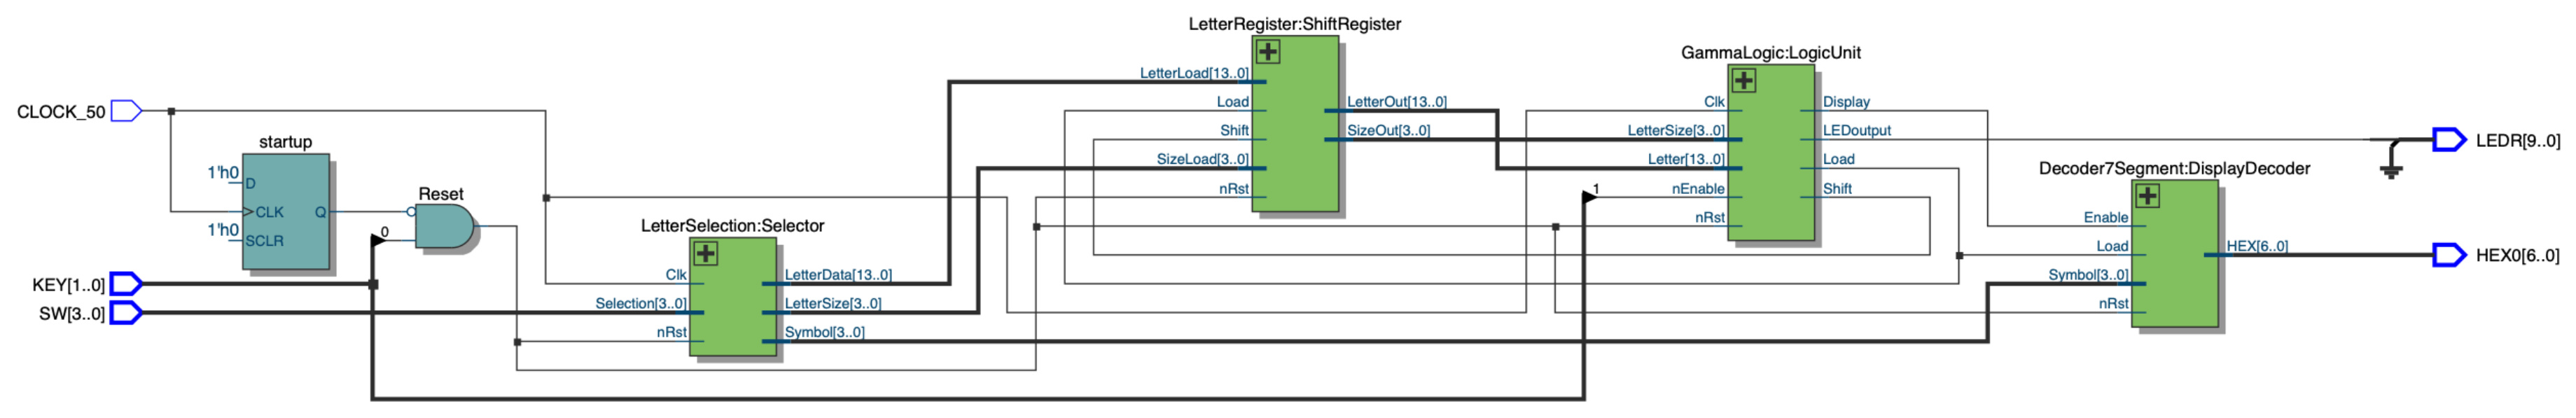
\includegraphics[width=1\textwidth]{Figures/RTL_TLE.jpg}
    \figcaption{RTL of the TLE}
    \label{fig:RTL_TLE}
\end{figure}

\clearpage

\begin{figure}[h]
    \centering
    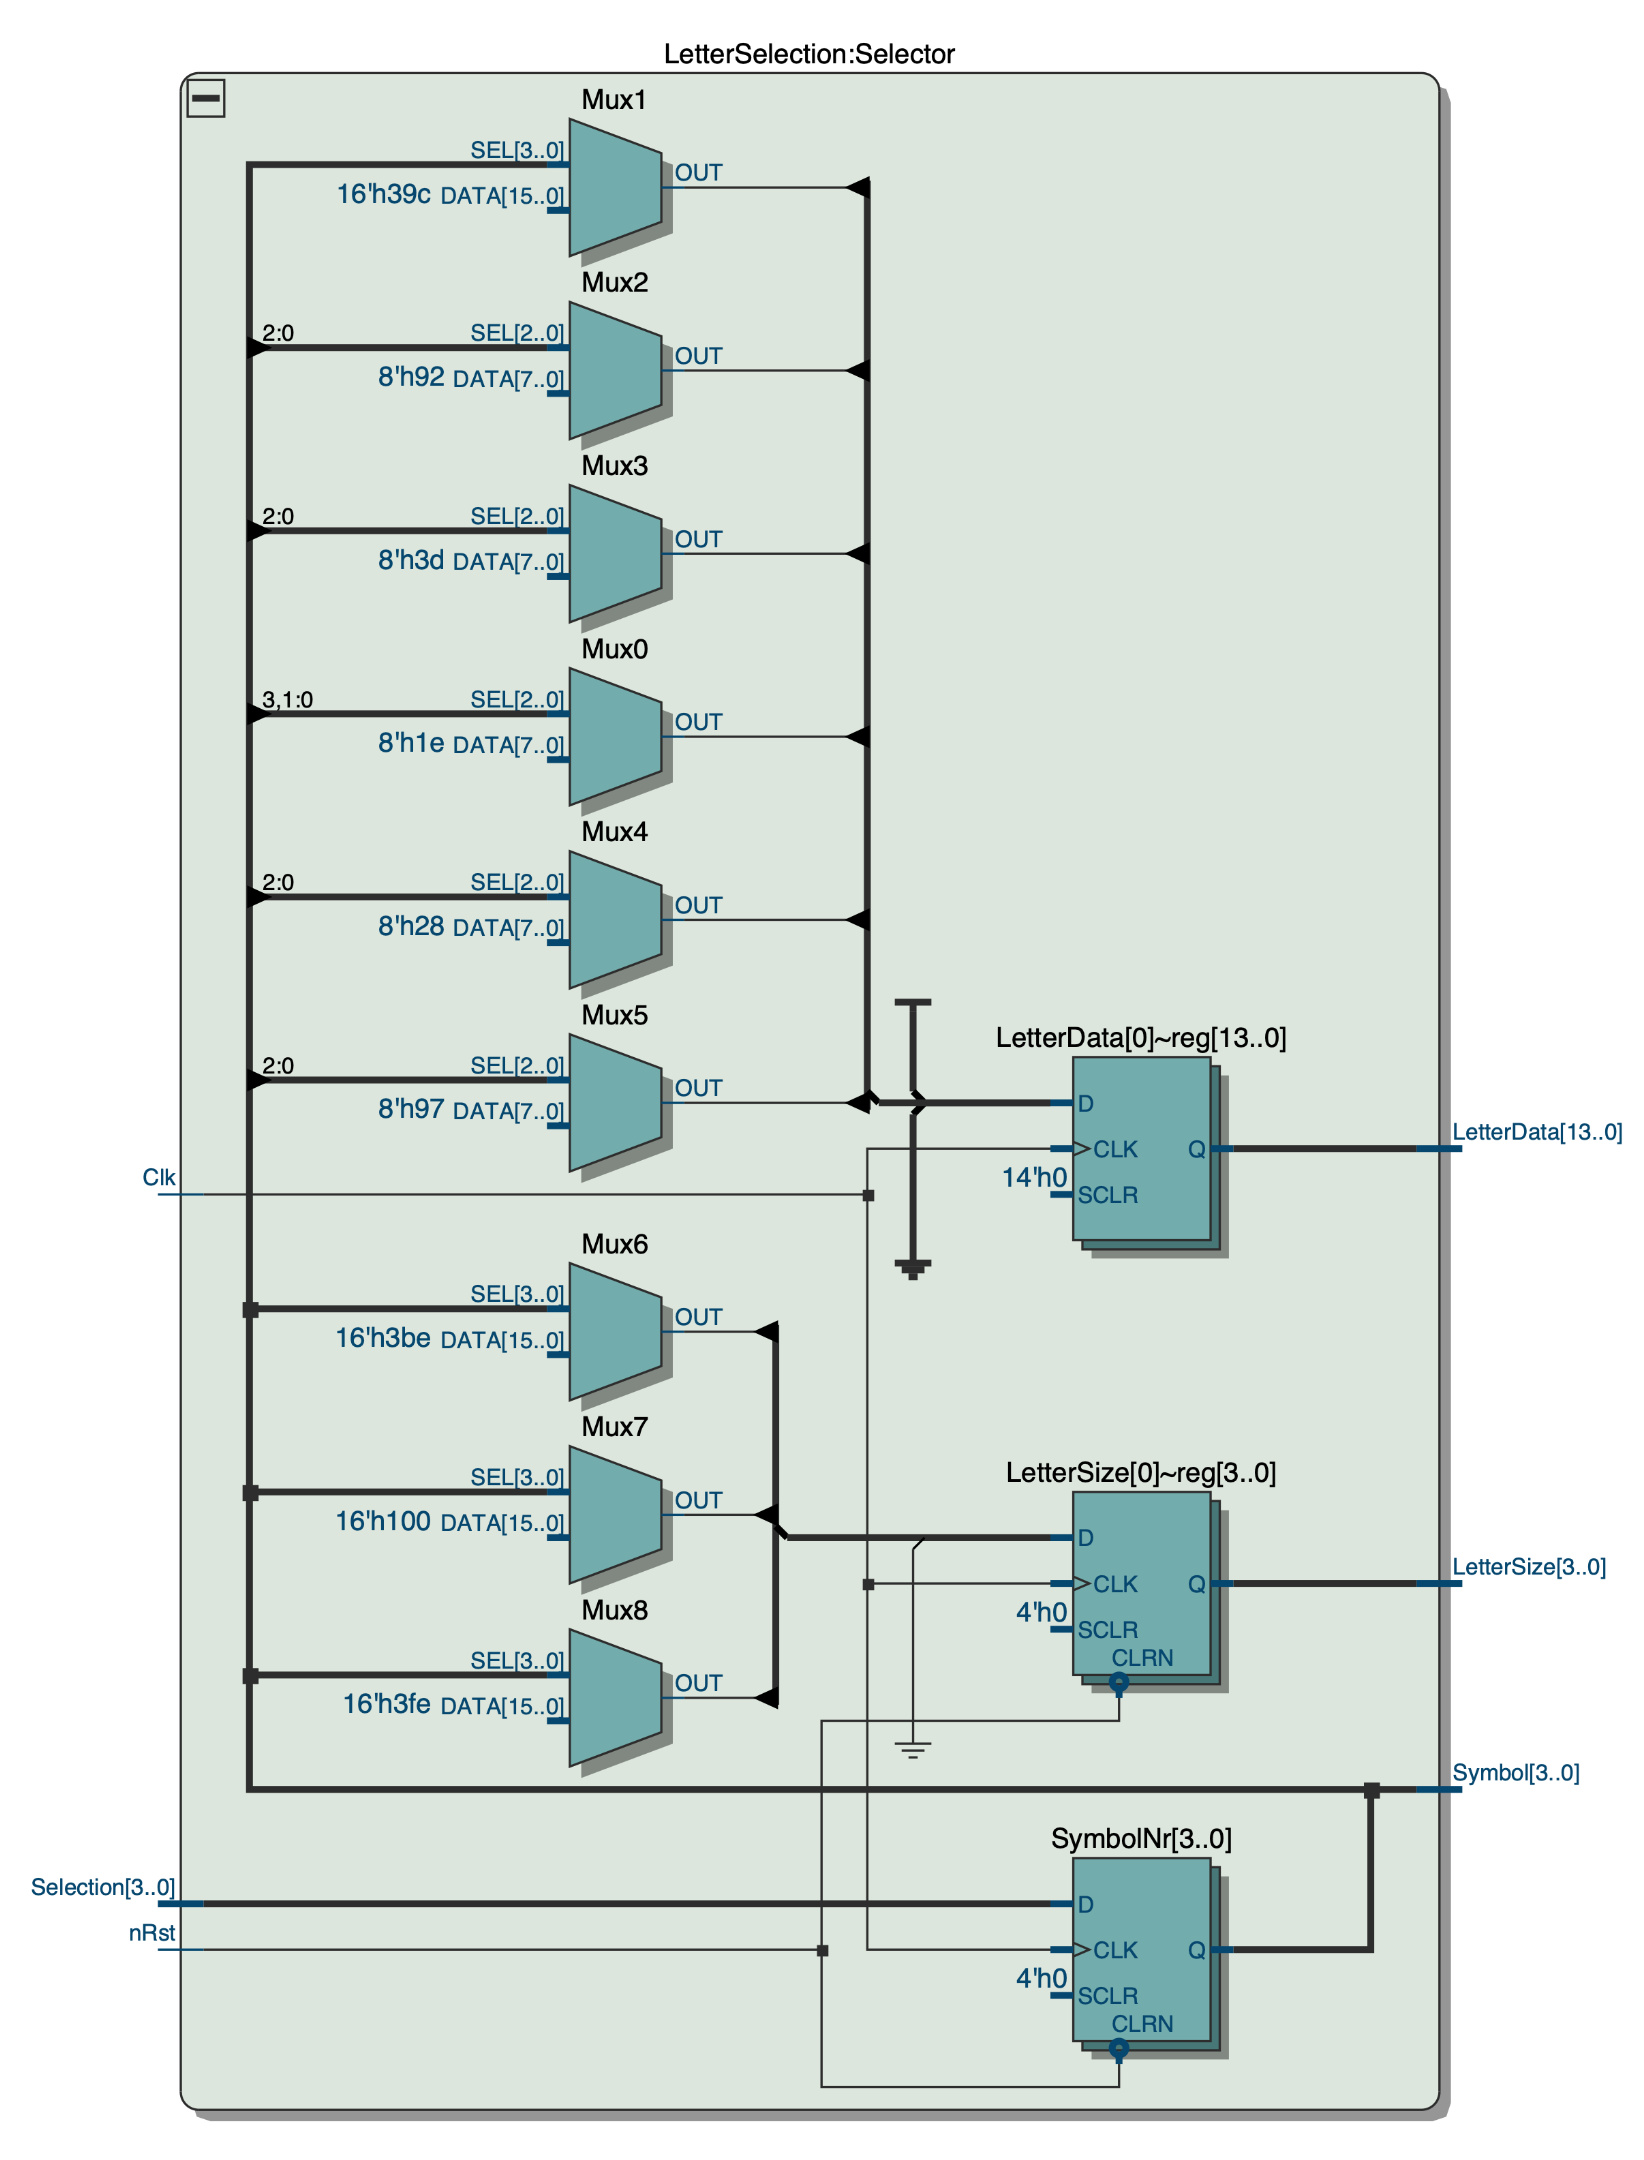
\includegraphics[width=1\textwidth]{Figures/RTL_Selector.jpg}
    \figcaption{RTL of the letter selector component}
    \label{fig:RTL_Sel}
\end{figure}

\clearpage

\begin{figure}[h]
    \centering
    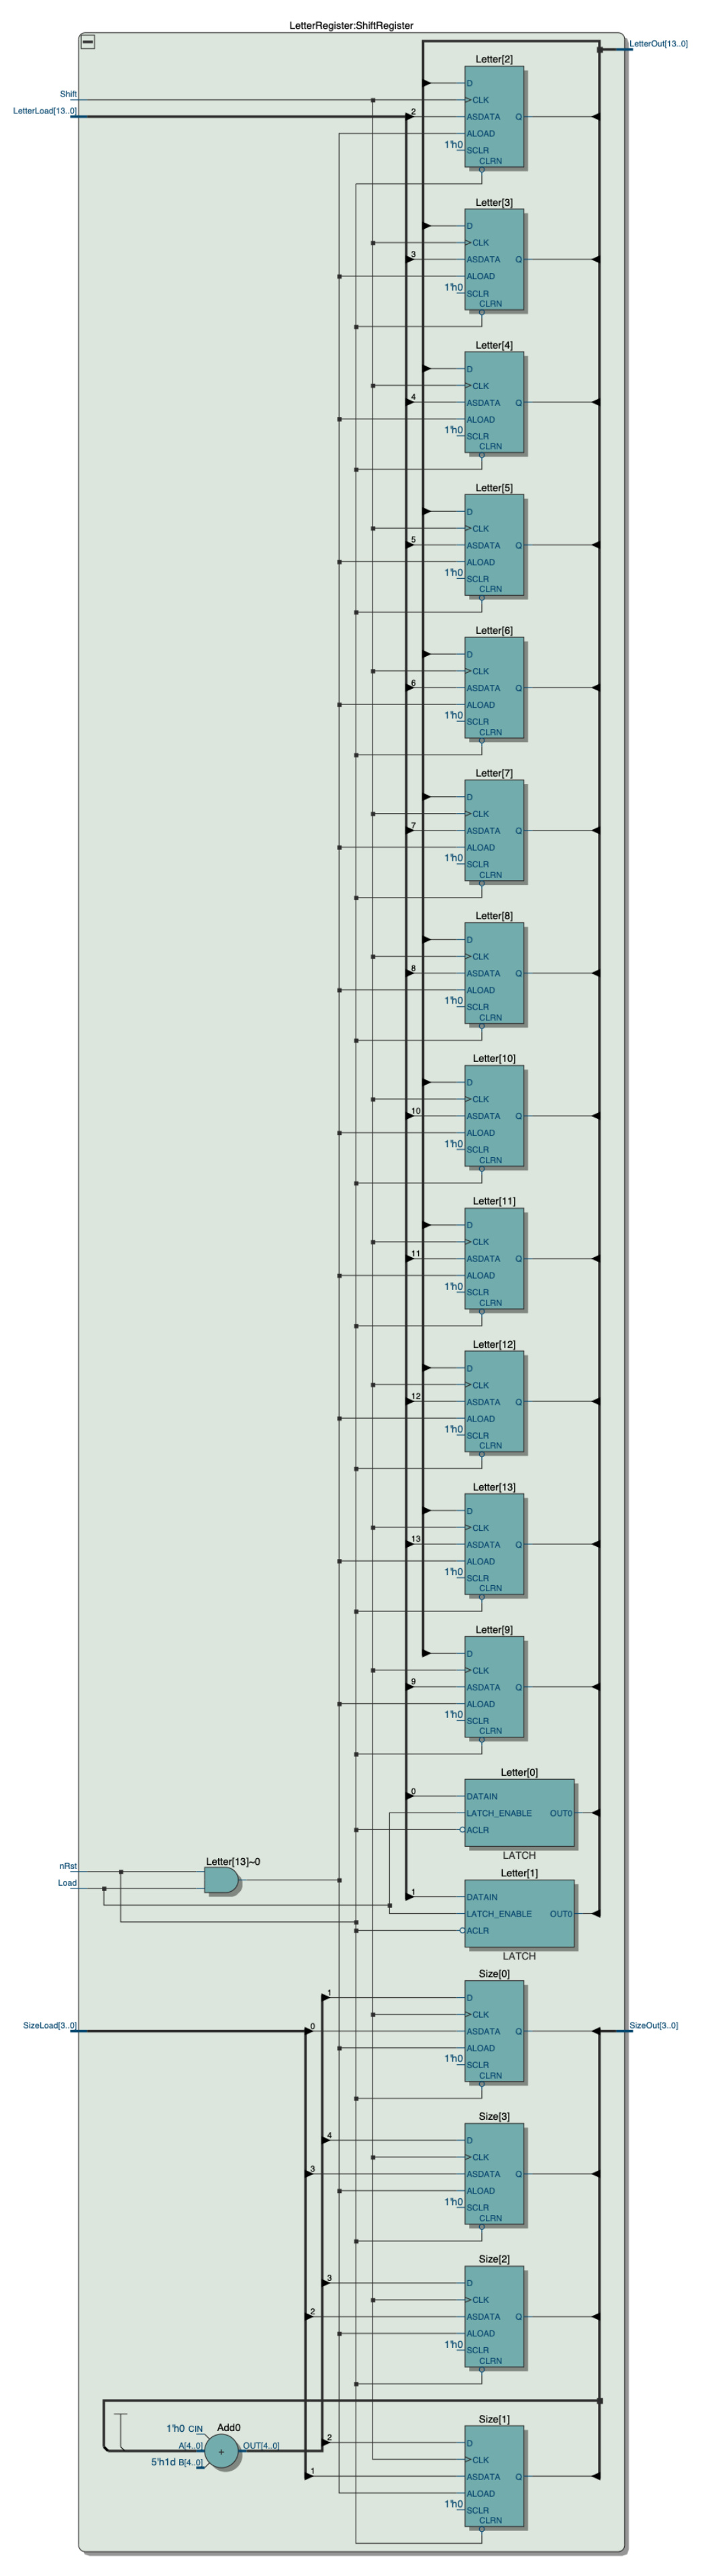
\includegraphics[width=0.4\textwidth]{Figures/RTL_Register.jpg}
    \figcaption{RTL of the letter shift register component}
    \label{fig:RTL_Reg}
\end{figure}

\clearpage

\begin{figure}[h]
    \centering
    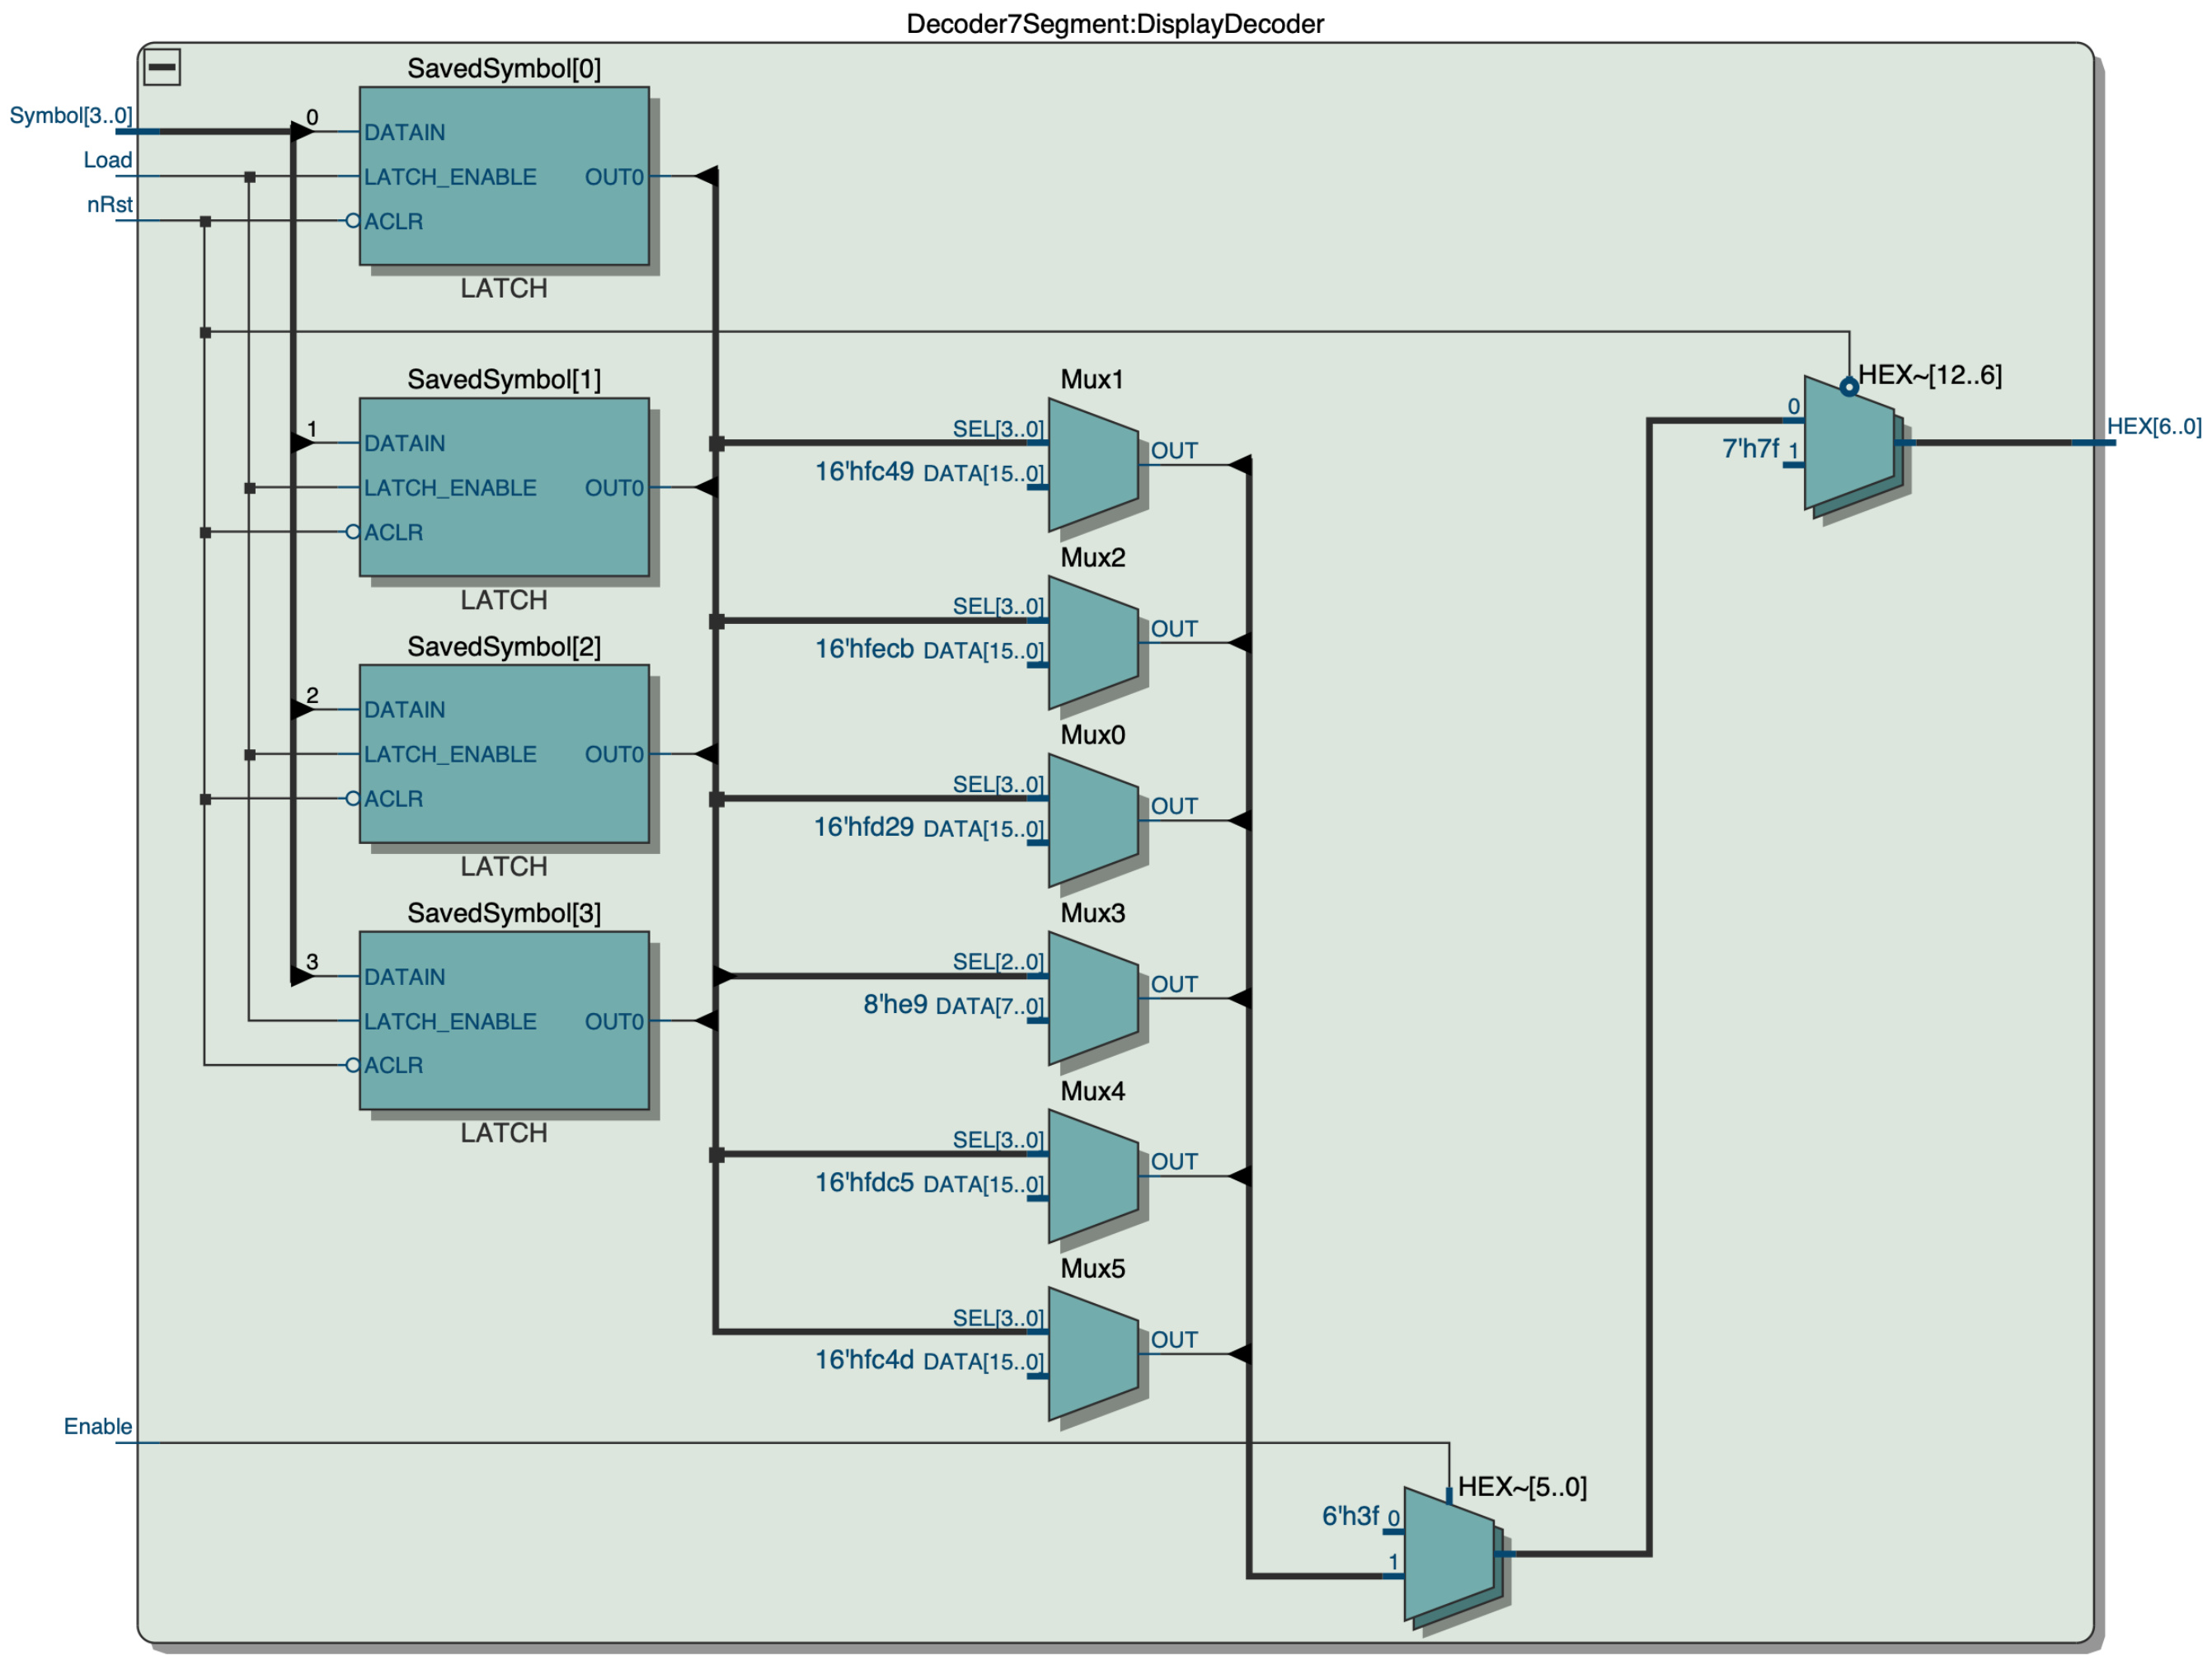
\includegraphics[width=1\textwidth]{Figures/RTL_Display.jpg}
    \figcaption{RTL of the 7 segment decoder component}
    \label{fig:RTL_Decoder}
\end{figure}

\begin{figure}[h]
    \centering
    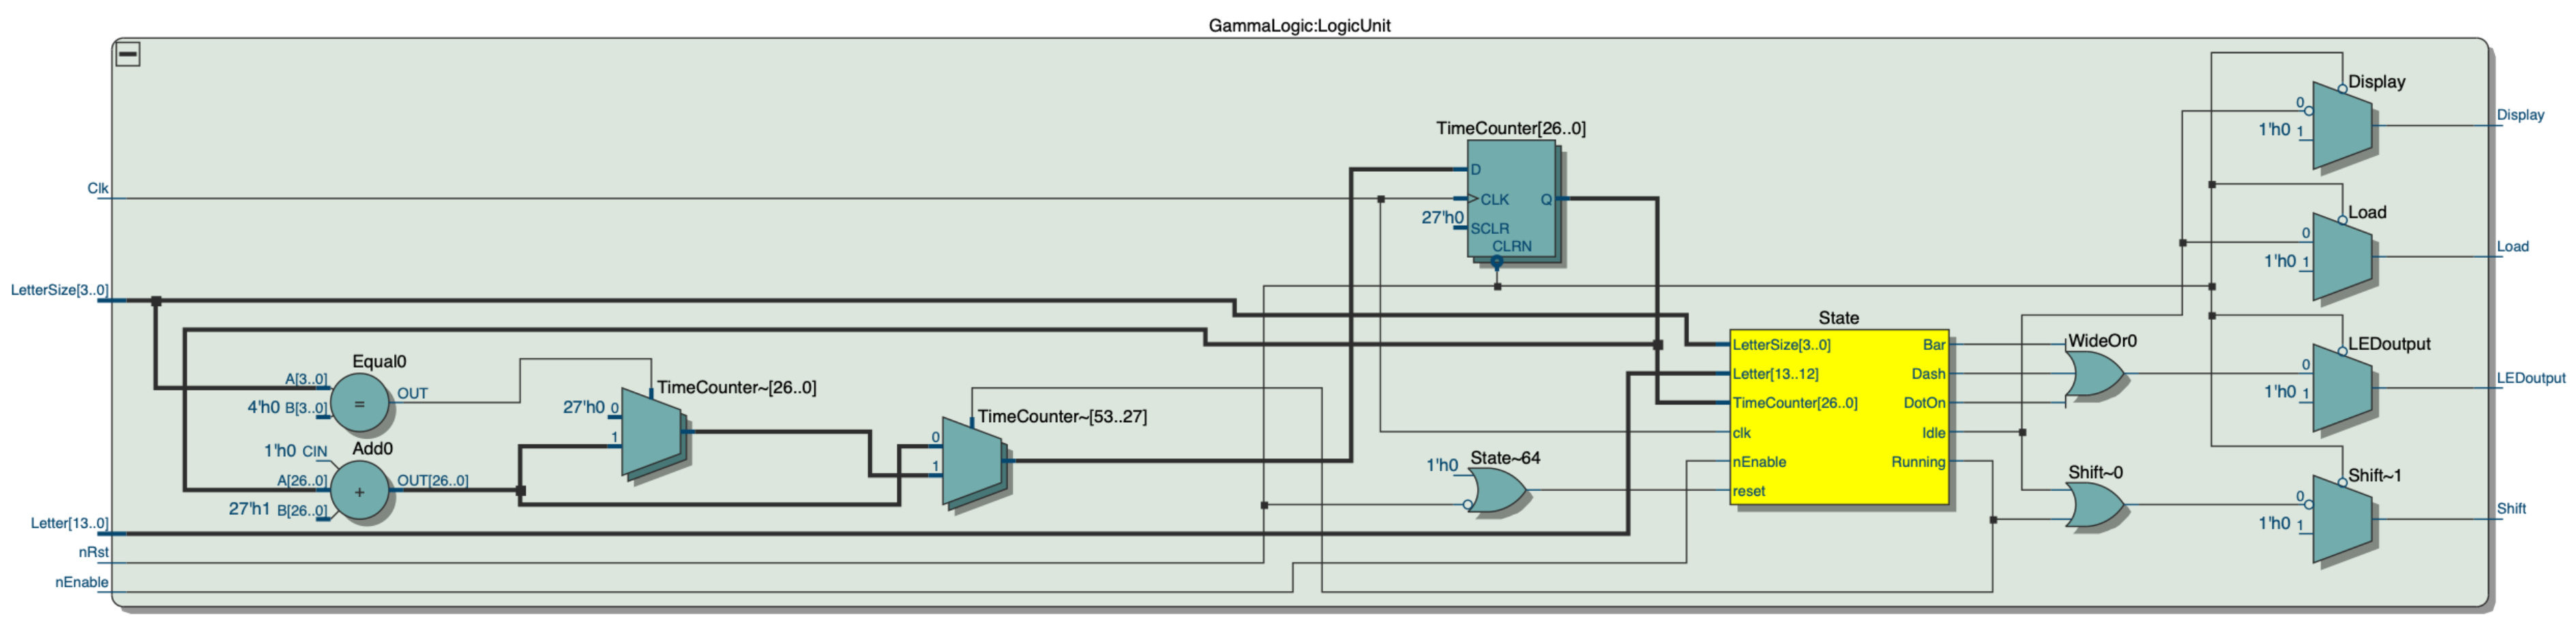
\includegraphics[width=1\textwidth]{Figures/RTL_Logic.jpg}
    \figcaption{RTL of the logic component}
    \label{fig:RTL_Logic}
\end{figure}

Quartus correctly recognizes that this is a FSM as seen in figure~\ref{fig:RTL_Logic} but it will not make a state transition diagram even though it is not that complex. Instead refer to the diagram in figure~\ref{fig:StateTransition}.

\clearpage
\subsection{Test bench code}
\writecode[VHDL]{LetterSelectionTB.vhd}{Testbench for the Letter selector}
\writecode[VHDL]{LetterRegisterTB.vhd}{Testbench for the Letter shift register}
\writecode[VHDL]{Decoder7SegmentTB.vhd}{Testbench for the 7 segment decoder}
\writecode[VHDL]{GammaLogicTB.vhd}{Testbench for the modified Logic control}
All test benches was made in a similar way. Testing both ordinary function and edge cases. Initially the test benches was much larger that the supplied code, this made for unreadable simulation results and therefore the test benches was simplified to the smallest amount of tests that could be done to be able to include the simulation results in this report.\par
The final testbench for the logic circuit also had a problem, it would just wait for at least 0.25s to move to the next state. This is unacceptable in a simulation tool. This is why a modified file is included, where the counter for the timer was reduced from counting up in the millions to at most 13. Here I represent 0.25s as two clock cycles instead of 125e5 cycles. There is no other change in code so this should work identical to the actual used code, only sped up for simulation purposes. For clarity sake the fast version is also included in the report and as a file.
\clearpage
\writecode[VHDL]{GammaLogicFast.vhd}{Logic control modified with a very small counter}


%   ############################## Section ##############################
\section{Results}

\subsection{Simulation}



\begin{figure}[h]
    \centering
    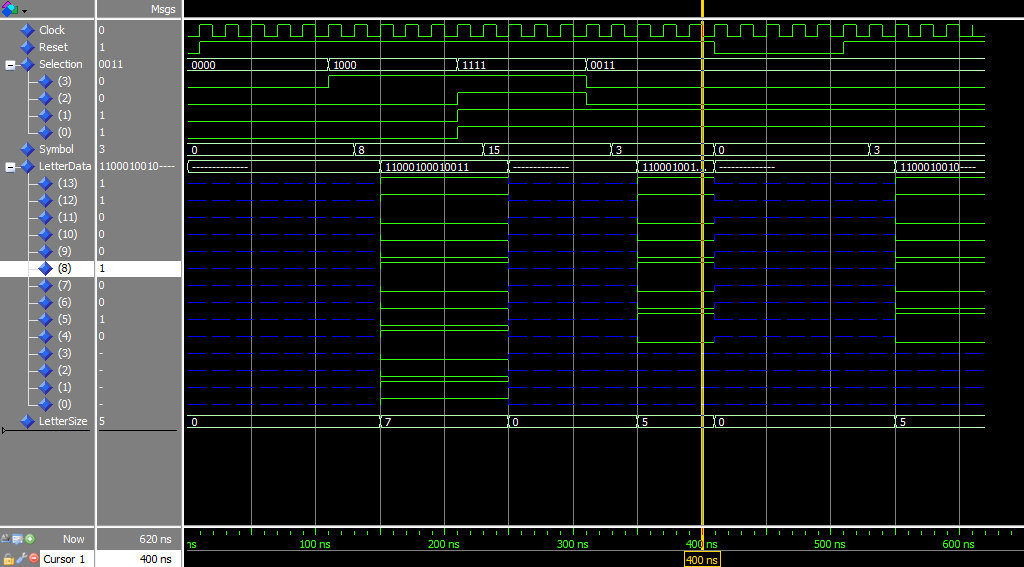
\includegraphics[width=1\textwidth]{Figures/LetterSelectorTB.PNG}
    \figcaption{TB Selector}
    \label{fig:TB_Sel}
\end{figure}
In this simulation it is clear to see that as long as reset is not pressed the value of Symbol, LetterData and LetterSize is following the input switches, with no delay for Symbol and one clock cycle for the others. This is because the 0th cycle upon changing the switches they are still read as old values, if in simulation these were changed only a single time unit before the clock edge rises it would be registers as the new value. on the 1st clock cycle after changing the value is read and stored in SymbolNr, then the instantly also saved in Symbol. The 2nd cycle is where the new saved value of SymbolNr is passing into the lookup table. This is because ModelSim simulates everything instantly for each time unit and therefore signal values don't change within a process like in traditional programming. When pressing the reset the value is instantly set no delay as it is asynchronous. 

\clearpage
\begin{figure}[h]
    \centering
    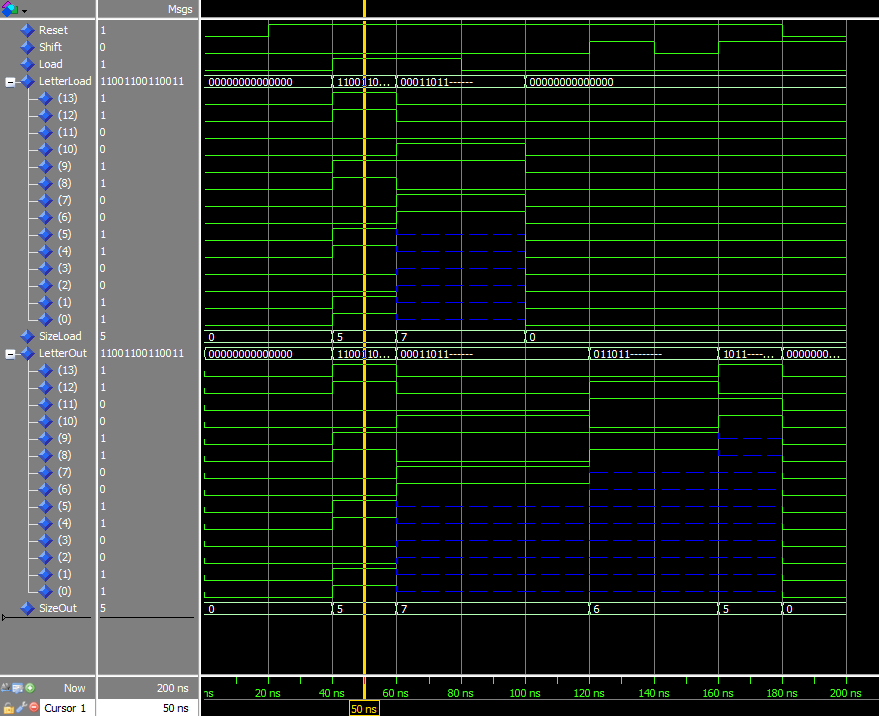
\includegraphics[width=1\textwidth]{Figures/LetterRegisterTB.PNG}
    \figcaption{TB Register}
    \label{fig:TB_Reg}
\end{figure}
In this simulation it is clear that when Load is high that it overrides current output instantly and when load is low again input values don't affect the output any more. It is also clear to see the shifting that happens on rising edge of Shift, where each time it adds the don't care and moves the values by two and counts down size by 1. The reset is asynchronous and clears output immediately when pressed.

\clearpage
\begin{figure}[h]
    \centering
    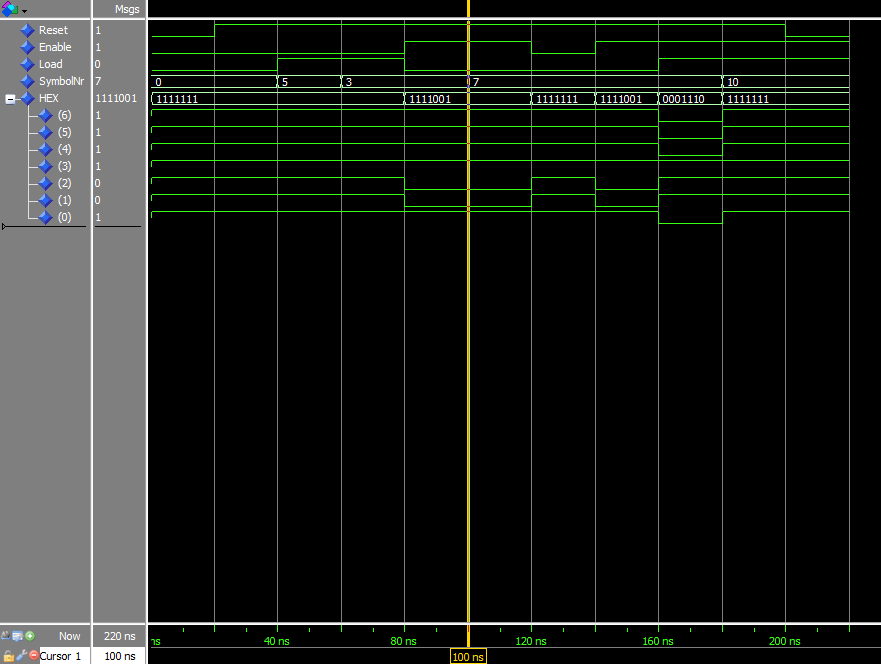
\includegraphics[width=1\textwidth]{Figures/DecoderTB.PNG}
    \figcaption{TB Decoder}
    \label{fig:TB_Decoder}
\end{figure}
In this simulation it is easy to see that the display is active whenever enable is high and not active when low. It is also possible to see how when Load is low and enable is high that it does not update the display. This is important as the display should remain the same regardless of switch positions throughout the sequence of symbols. Enable and Load are outputs from the FSM and is technically just not gated from the other, this means that the display should never change midway as it never goes to Idle unless done.

\clearpage
\begin{figure}[h]
    \centering
    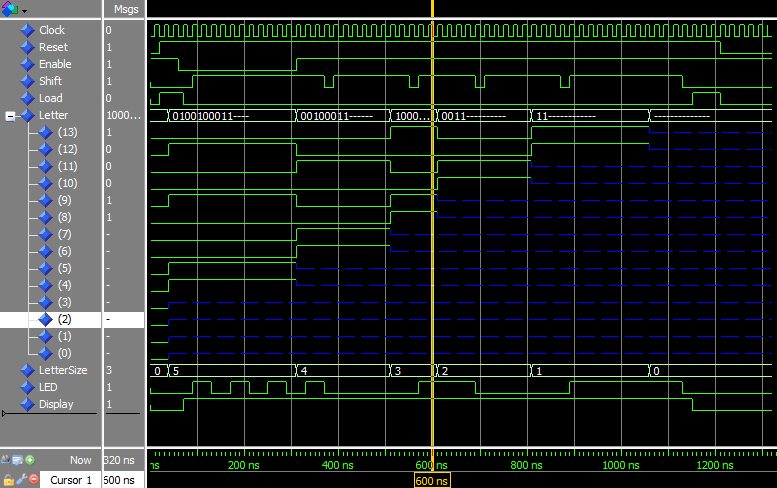
\includegraphics[width=1\textwidth]{Figures/LogicTB.PNG}
    \figcaption{TB Logic}
    \label{fig:TB_Logic}
\end{figure}
This is the most interesting simulation where at the bottom the dot, dash, bar and between can easily be observed. This is only possible because of simulating using the counter modified logic code. Looking at enable, the start sending keypress, it activates the logic sequence to happen and the FSM moves along and shifts the LetterData as it goes. This shifting of data is done manually in the test bench as the logic is not connected to the shift register during the test bench. At the end it goes back to the idle state, signified by load being turned high. And when pressing reset all outputs are set to zero.

\subsection{Implementation}
Implementation was done on the FPGA board and a video file uploaded showing it working as intended trying every combination and some more.

%   ############################## Section ##############################
\section{Conclusion}
In the end I learned a lot from doing this Project. I also felt a high level of understanding and mastery as I was able to write all the code in its entirety without any simulation or compilation and only trying to compile it 7 times and fixing minor errors such as missing semicolons or reserved names before it worked as intended, with no change to the actual logic. I think there are a few areas of improvement that can be done with my code. I think removing the 00 for between in the LetterData and maybe have a boolean for "have waited" true or false, that would be false when returning to running from a symbol state and after being in the between state it goes to true and is then proceed to the next symbol state. This would also have to be true when coming from idle to not introduce a start delay, and it needs to be checked after size is checked to not add end delay. Other improvements I have thought about is cleaning up the code. I have tried to make the code as clean as possible but I still fell like the signal names and module names are not the most intuitive names and could be a bit confusing. The final improvement that could be made is to remove the timer counter from the logic and make a resettable ticker counter that gives a 1 cycle synchronous pulse that can be read by the state transition logic. Then the Running state could reset it whenever initiated and use a small counter to keep track of each states length. Although I am on the fence about that as I like that having it clocked to 50MHz is for circuits like this essentially the same as having actions happen instantly. There is no input delay and transitions happen immediately, unlike a 4Hz clock where if timed bad could give a "whole" 0.249s input delay, maybe this even causes the input to not register if fast enough. All in all I am happy with the way I solved the task and how the code works and I personally don't think I can improve it by much without adding other problems or complications that makes it not as clean of a result. "In anything at all, perfection is finally attained not when there is no longer anything to add, but when there is no longer anything to take away, when a body has been stripped down to its nakedness." by Antoine de Saint-Exupery. This is a quote I really like and try to think about when designing anything such that it functions in the most simple and elegant way I can think of. I am by no means saying this code is absolute perfection, but it in my vision it cannot be simplified any more to my knowledge and thereby I am happy about my design.

\end{document}
